\chapter{anexos}

\section{VIs do ator de comunicação serial}

        \begin{figure}
                \centering
                 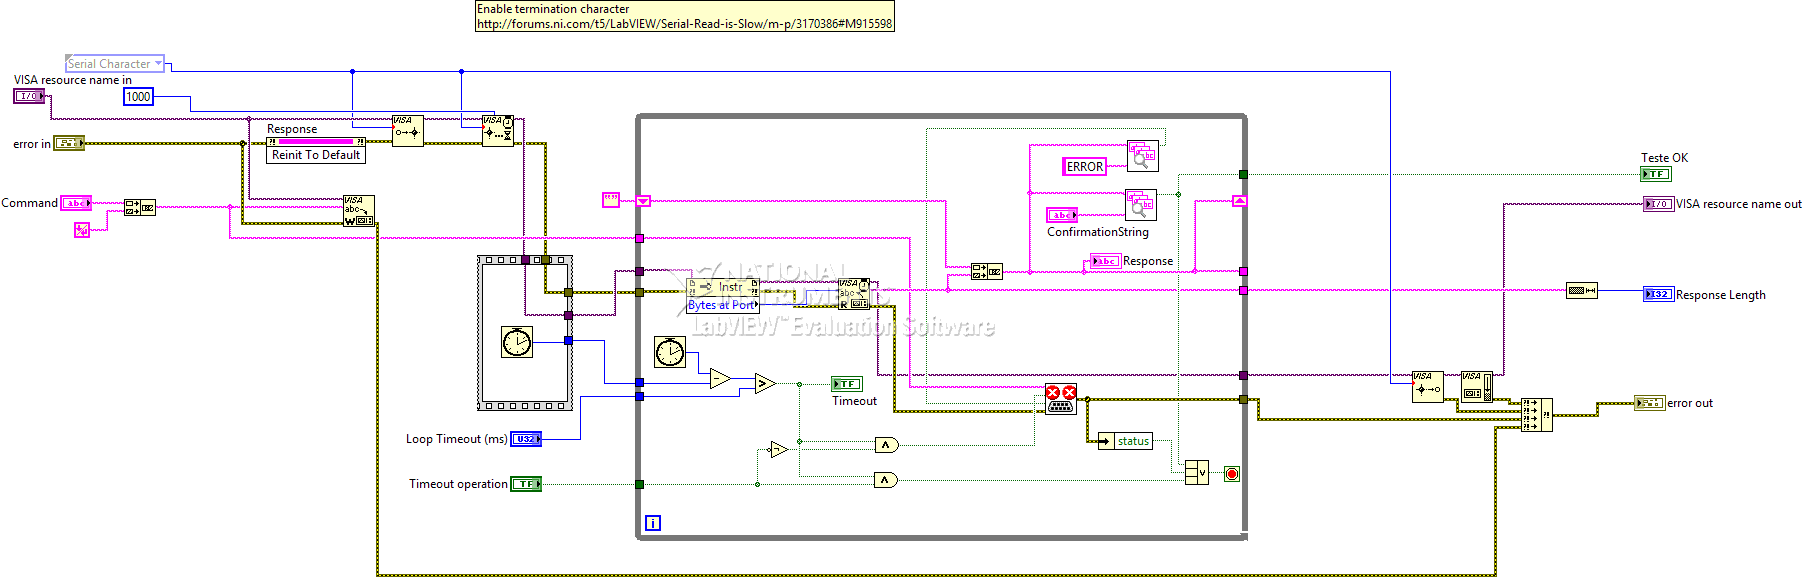
\includegraphics[width=1\linewidth]{lv/modcom/ModCOM_serialcored}
                \caption{Captura de tela da função básica de teste serial}
                \label{fig:serialcored}
        \end{figure}
        
        \begin{figure}
                \centering
                 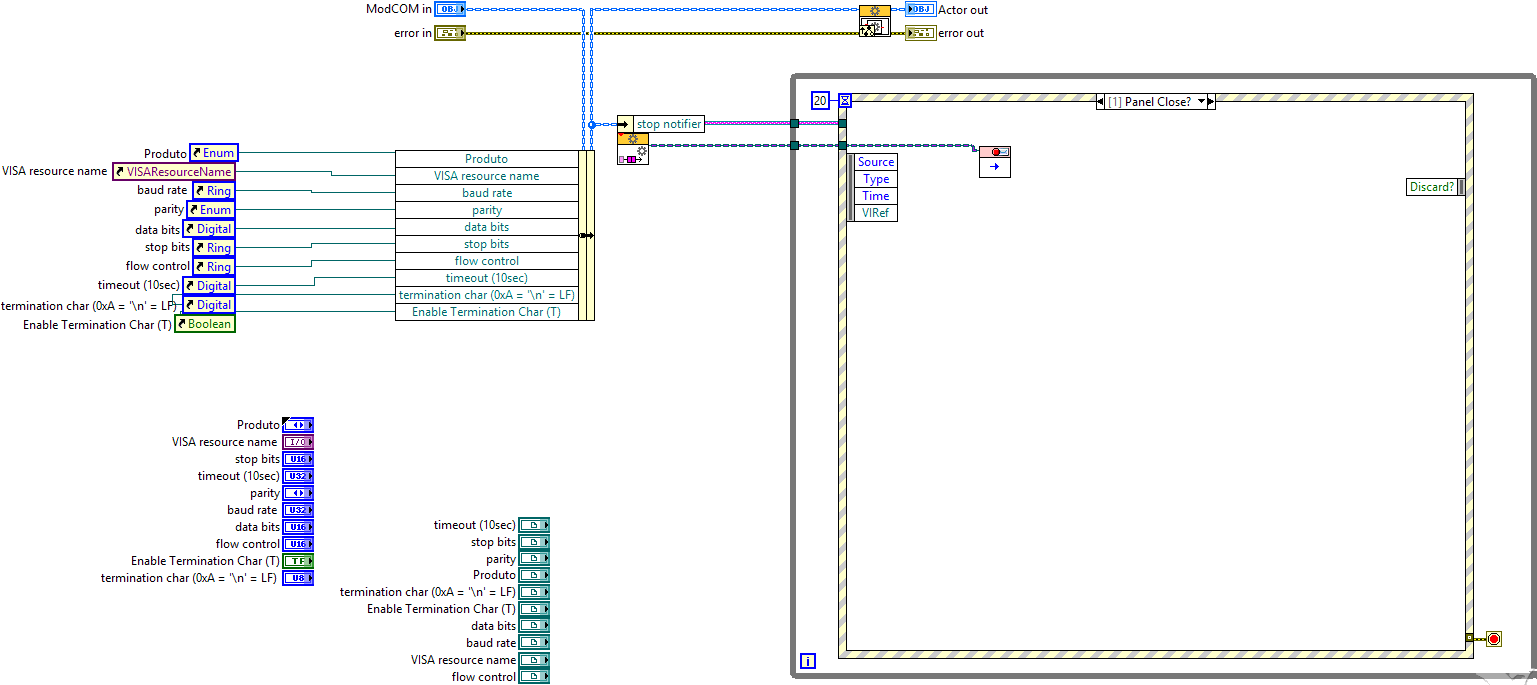
\includegraphics[width=1\linewidth]{lv/modcom/ModCOM_lvclass_Actor_Cored}
                \caption{Captura de tela do Actor Core do comunicador serial}
                \label{fig:modcomcore}
        \end{figure}
        
        \begin{figure}
                \centering
                 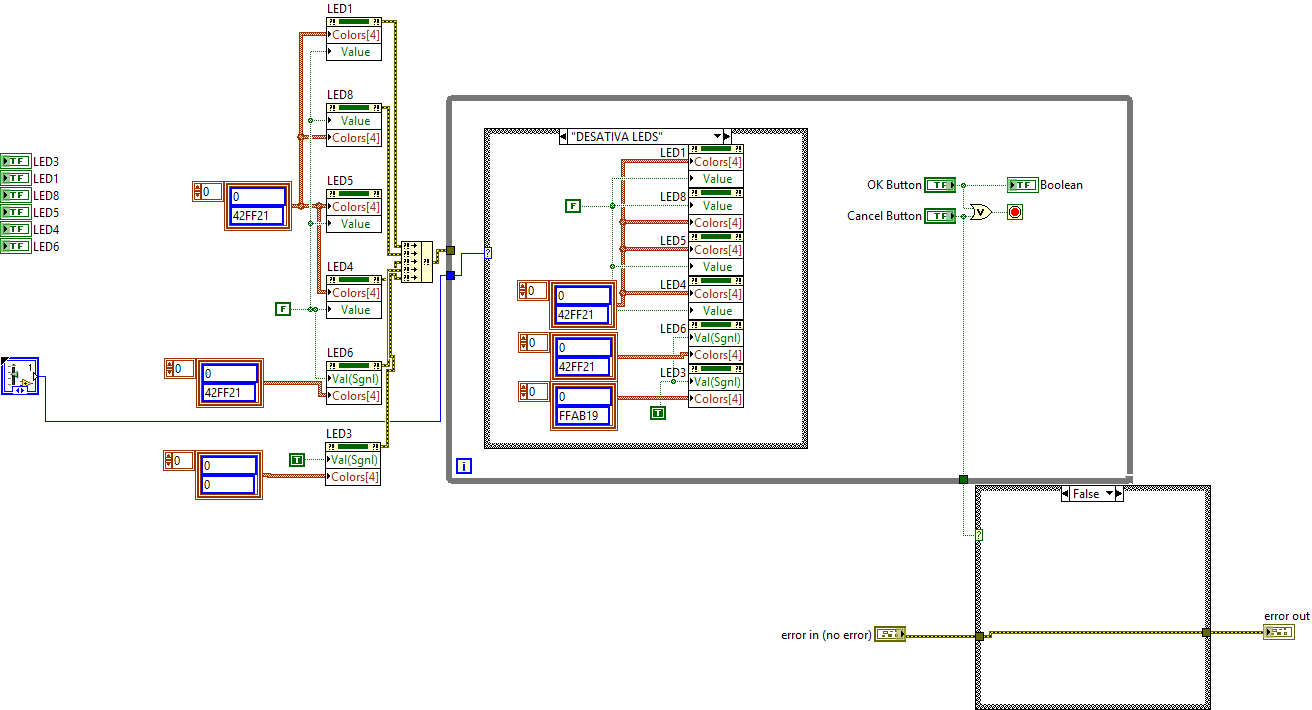
\includegraphics[width=1\linewidth]{lv/modcom/ModCOM_LED_popupd}
                \caption{Captura de tela do Diagrama de Blocos da rotina de testes de LEDs e GPIOs}
                \label{fig:modcomledd}
        \end{figure}
        
        
        
        \begin{figure}
                \centering
                 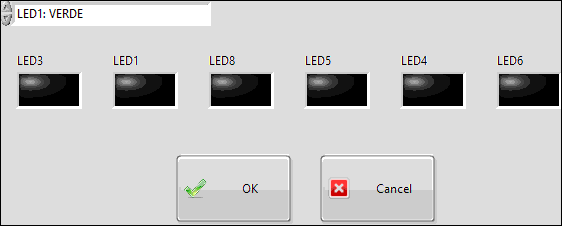
\includegraphics[width=1\linewidth]{lv/modcom/ModCOM_LED_popupp}
                \caption{Captura de tela do Painel Frontal de testes de LEDs e GPIOs}
                \label{fig:modcomledp}
        \end{figure}
        % parte oculta de diagramas
    \begin{comment}
        
         \begin{figure}
                \centering
                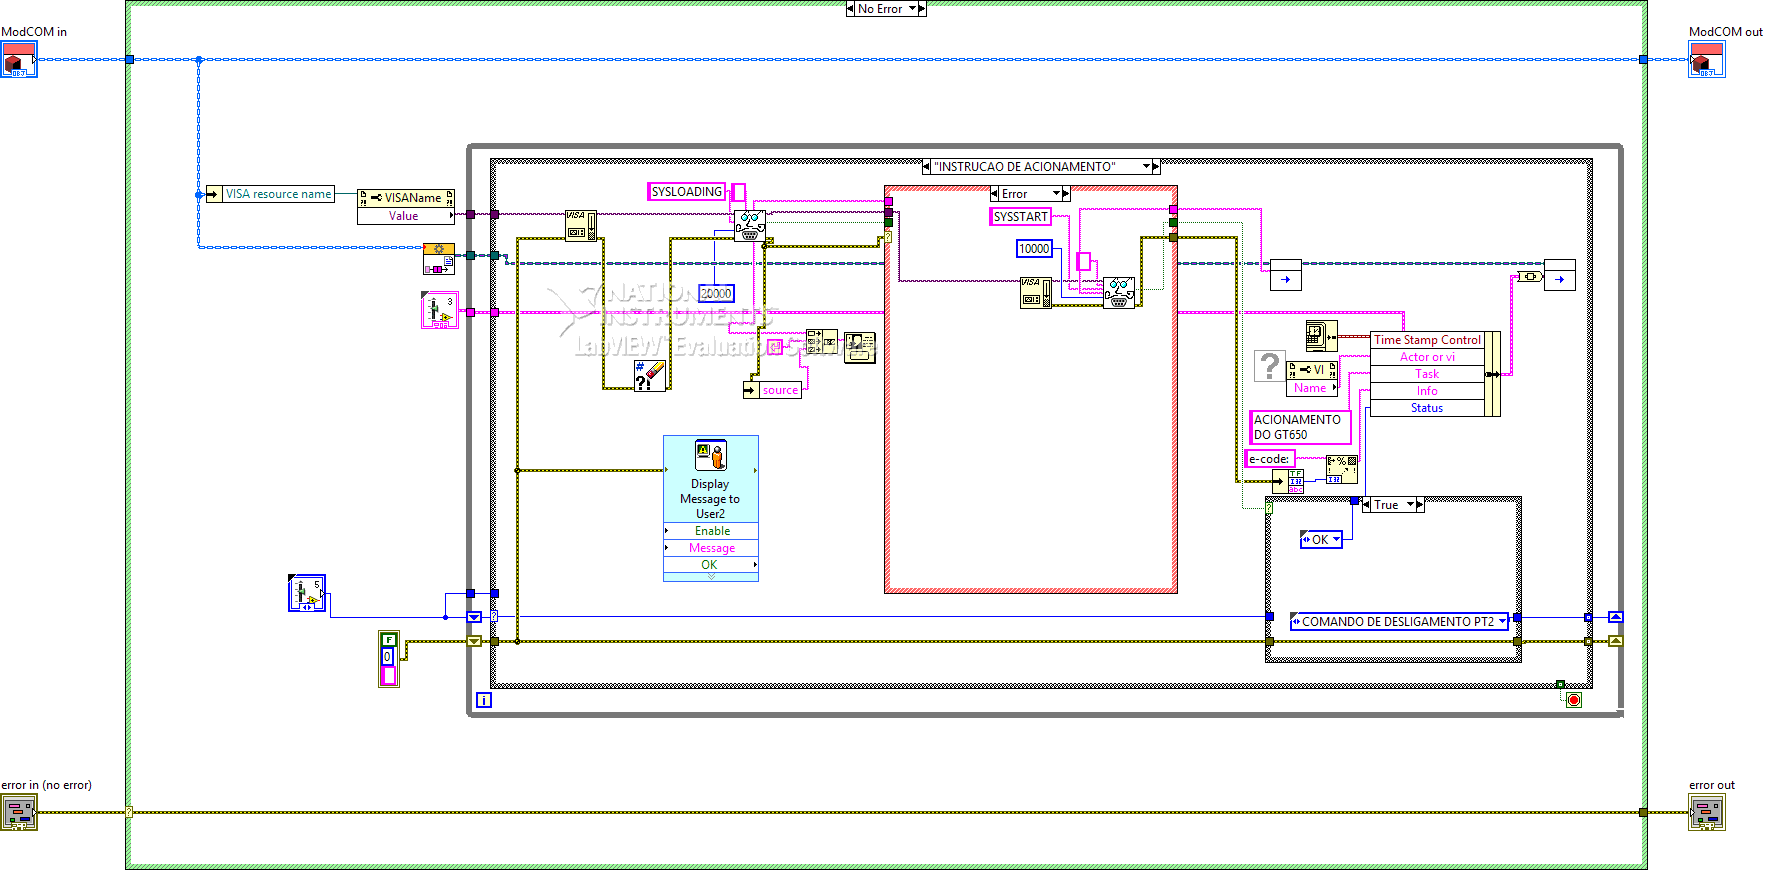
\includegraphics[width=1\linewidth]{lv/modcom/ModCOM_lvclass_desligamentoresetd}
                \caption{Captura de tela do Rotina de desligamento e reset do modem}
                \label{fig:modcomshutdown}
        \end{figure}
        
        
        \begin{figure}
                \centering
                 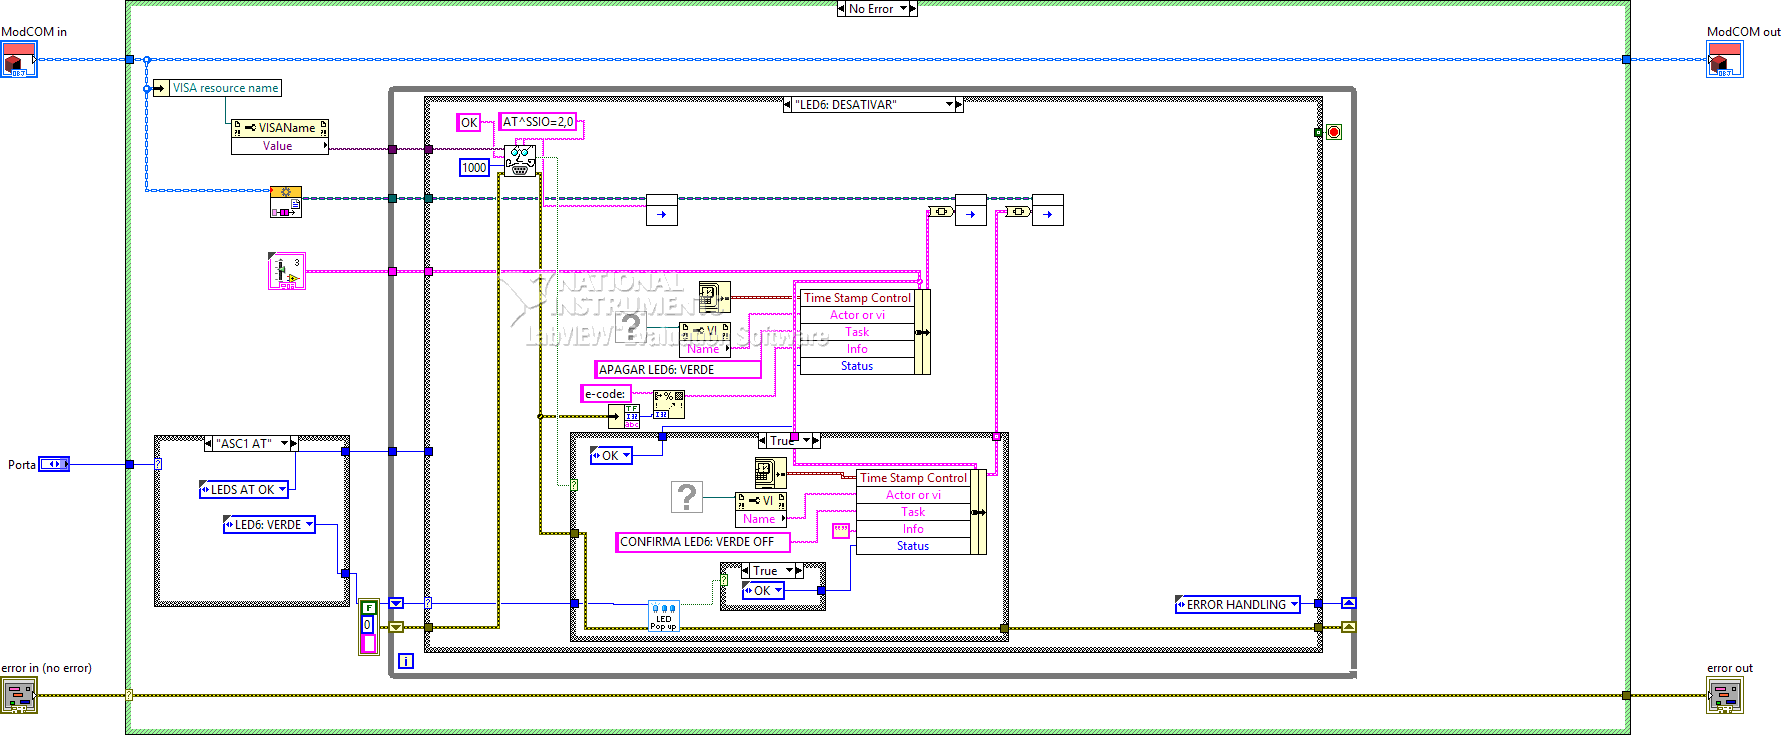
\includegraphics[width=1\linewidth]{lv/modcom/ModCOM_LED_I2Cd}
                \caption{Captura de tela do comunicador i2c}
                \label{fig:modcomledi2c}
        \end{figure}
        
        
        \begin{figure}
                \centering
                 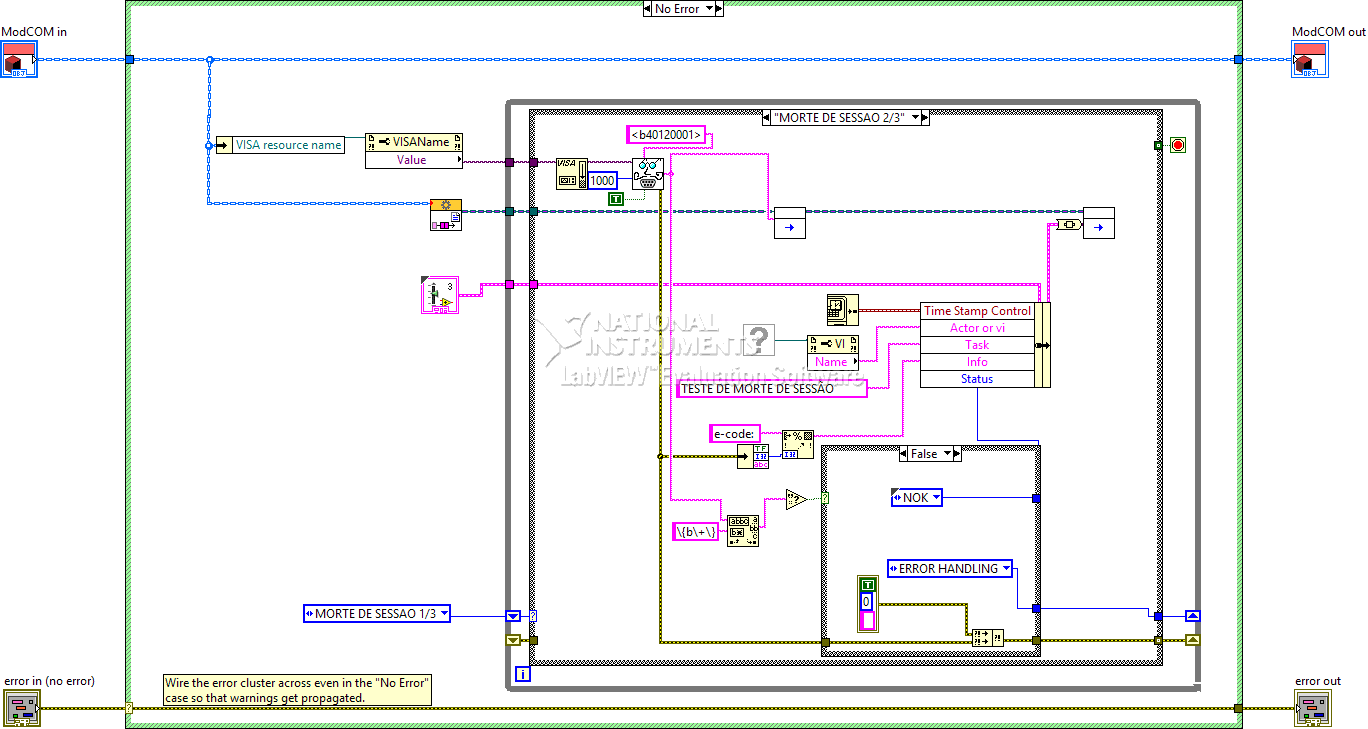
\includegraphics[width=1\linewidth]{lv/modcom/ModCOM_morted}
                \caption{Captura de tela do Teste de fechamento ou morte de comunicação serial}
                \label{fig:modcommorte}
        \end{figure}
        
        \begin{figure}
                \centering
                 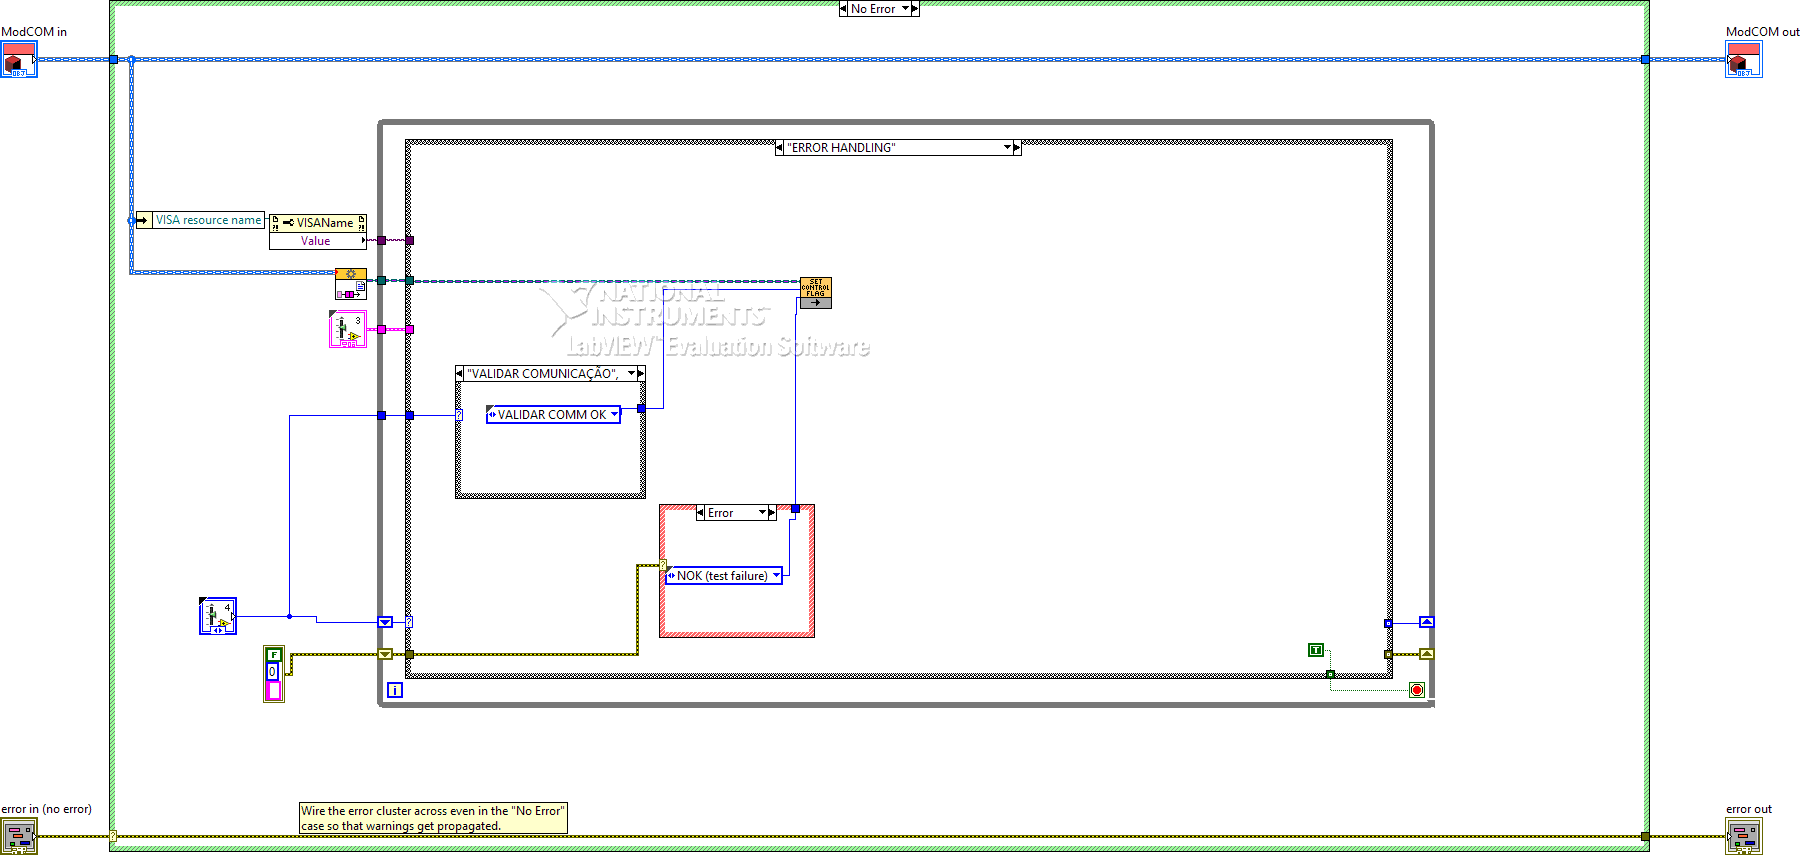
\includegraphics[width=1\linewidth]{lv/modcom/ModCOM_nopsutestd}
                \caption{Captura de tela do Captura de tela da rotina de teste sem fonte de alimentação}
                \label{fig:modcomnopsu}
        \end{figure}
        
        \begin{figure}
                \centering
                 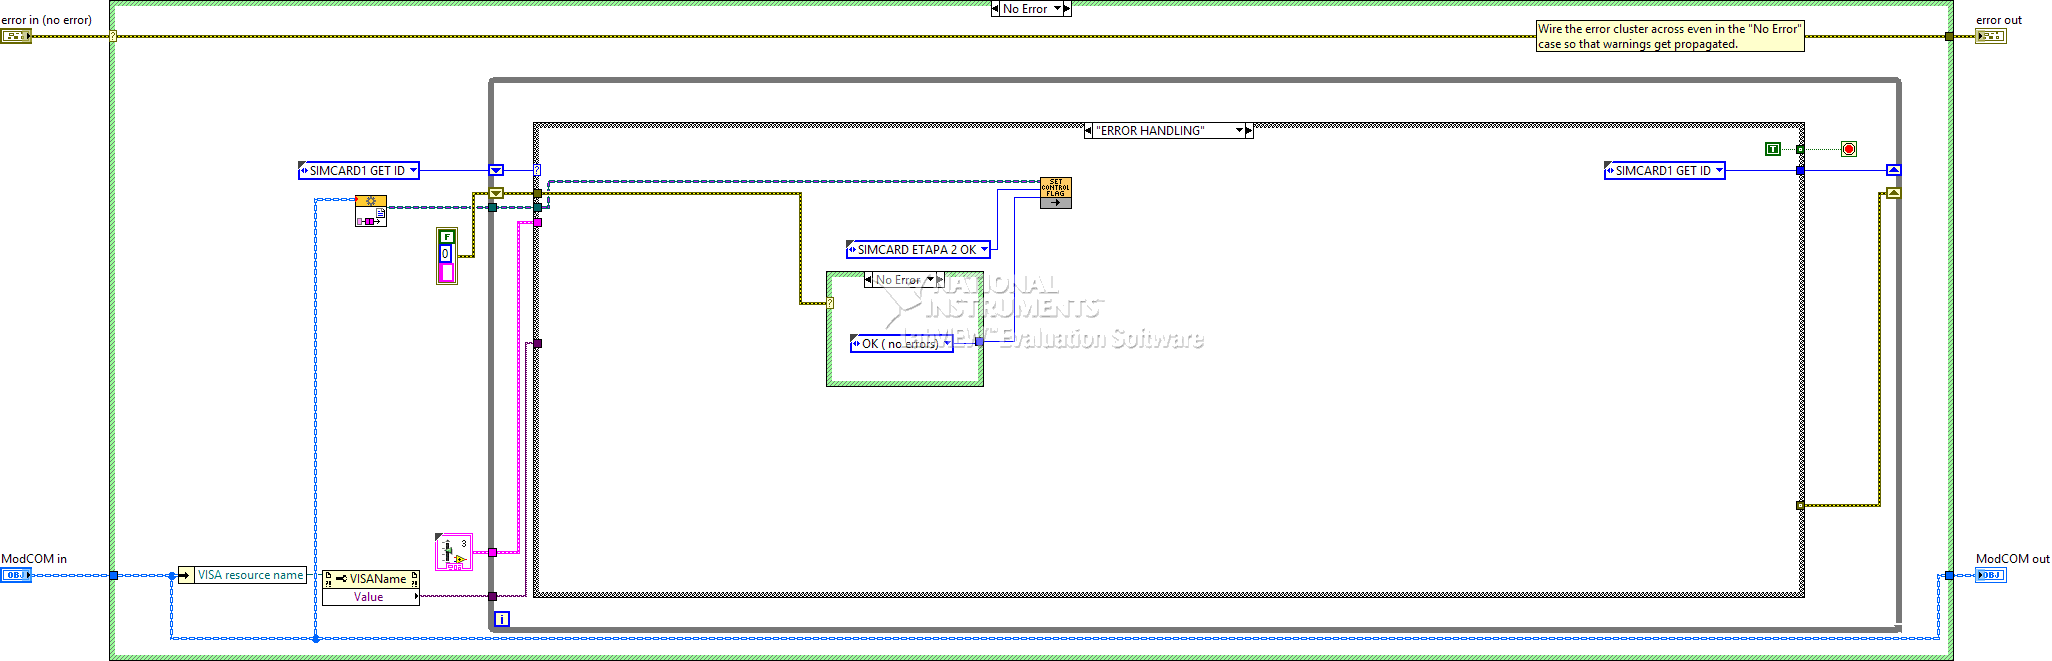
\includegraphics[width=1\linewidth]{lv/modcom/ModCOM_simcard}
                \caption{Captura de tela da rotina de teste dos simcard}
                \label{fig:modcomsimcard}
        \end{figure}
        
        \begin{figure}
                \centering
                 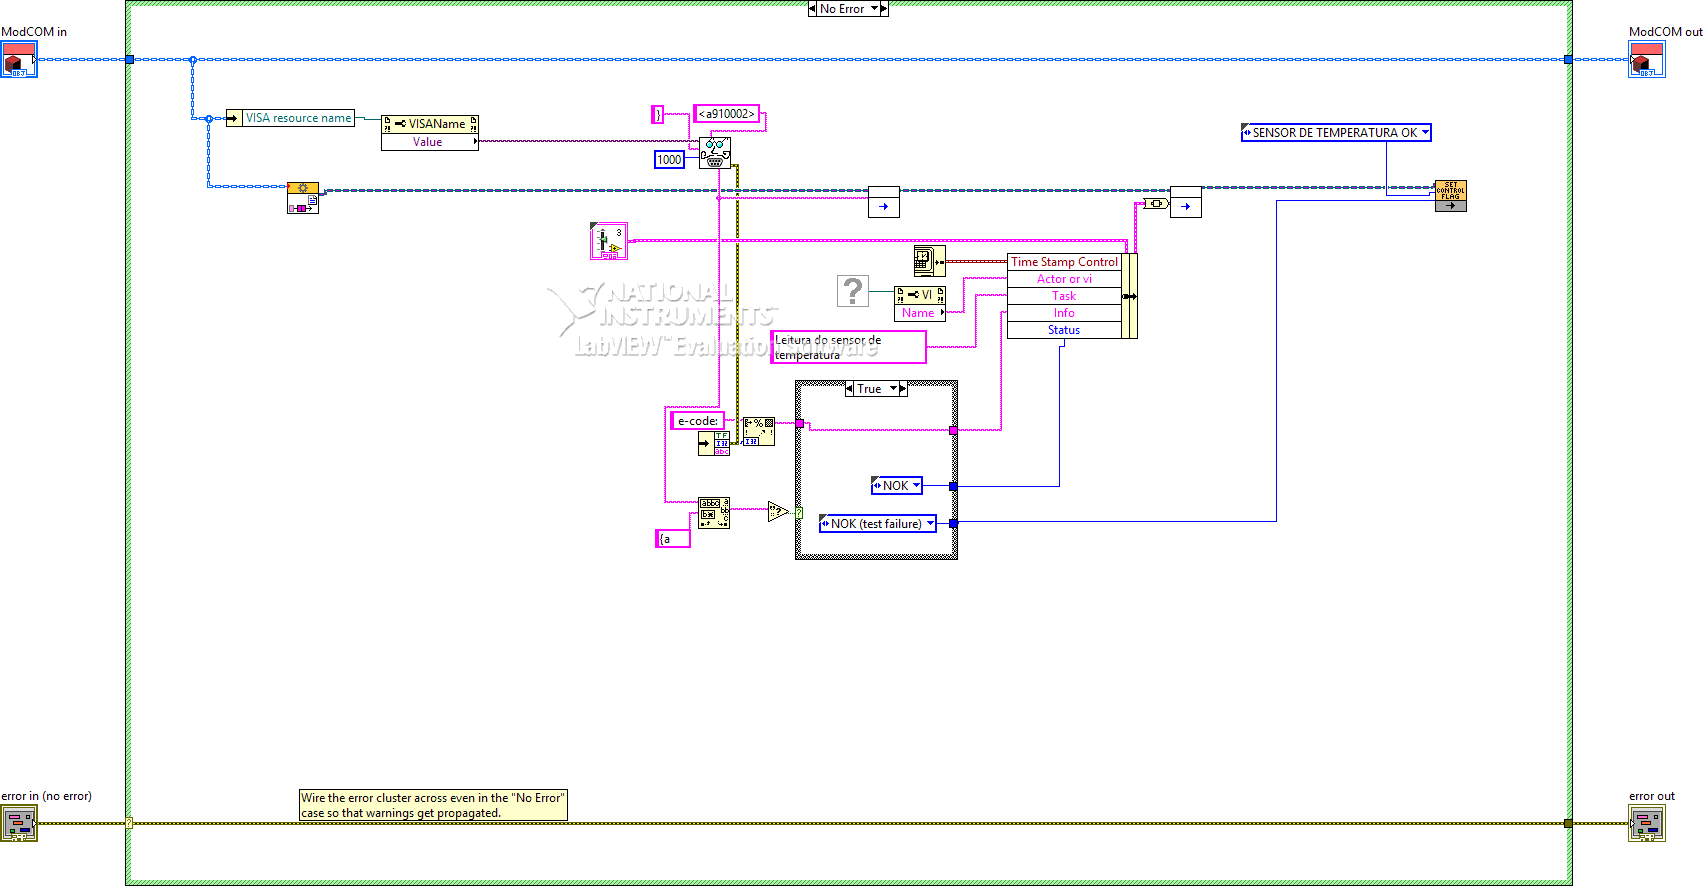
\includegraphics[width=1\linewidth]{lv/modcom/ModCOM_temp}
                \caption{Captura de tela da rotina de teste do sensor de temperatura}
                \label{fig:modcomtemp}
        \end{figure}
        
        
        \begin{figure}
                \centering
                 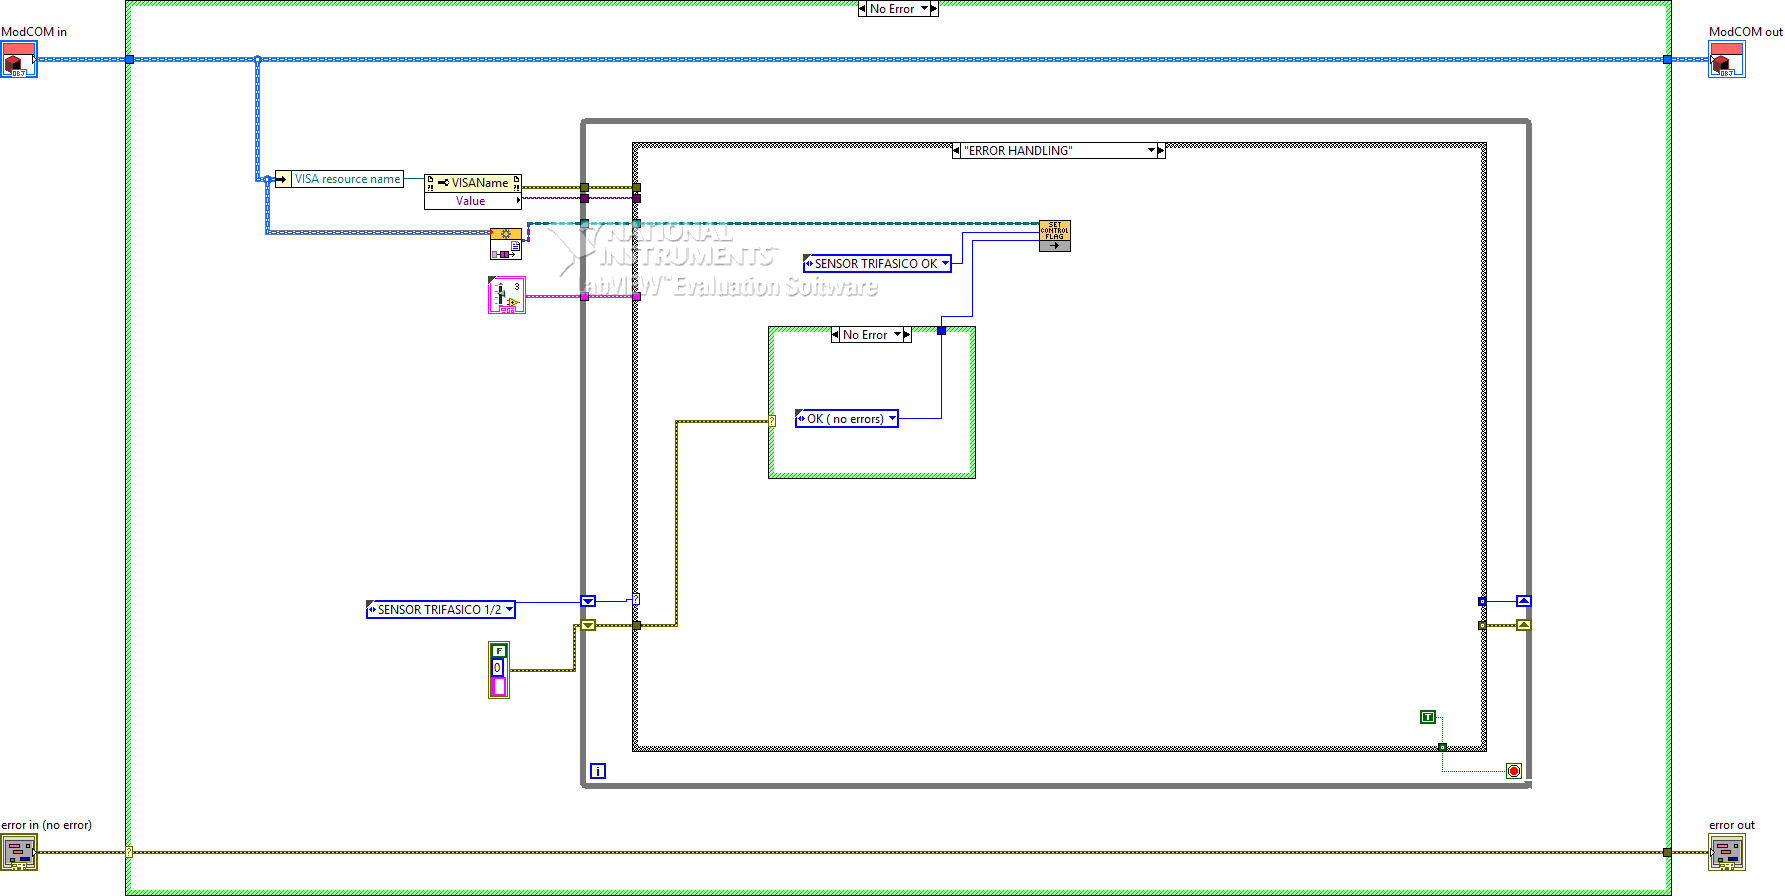
\includegraphics[width=1\linewidth]{lv/modcom/ModCOM_tritestd}
                \caption{Captura de tela da rotina de teste do sensor de presença das tensões trifásicas}
                \label{fig:modcomtri}
        \end{figure} 
    \end{comment}
    
\section{VI do ator controlador}

       \begin{figure}
                \centering
                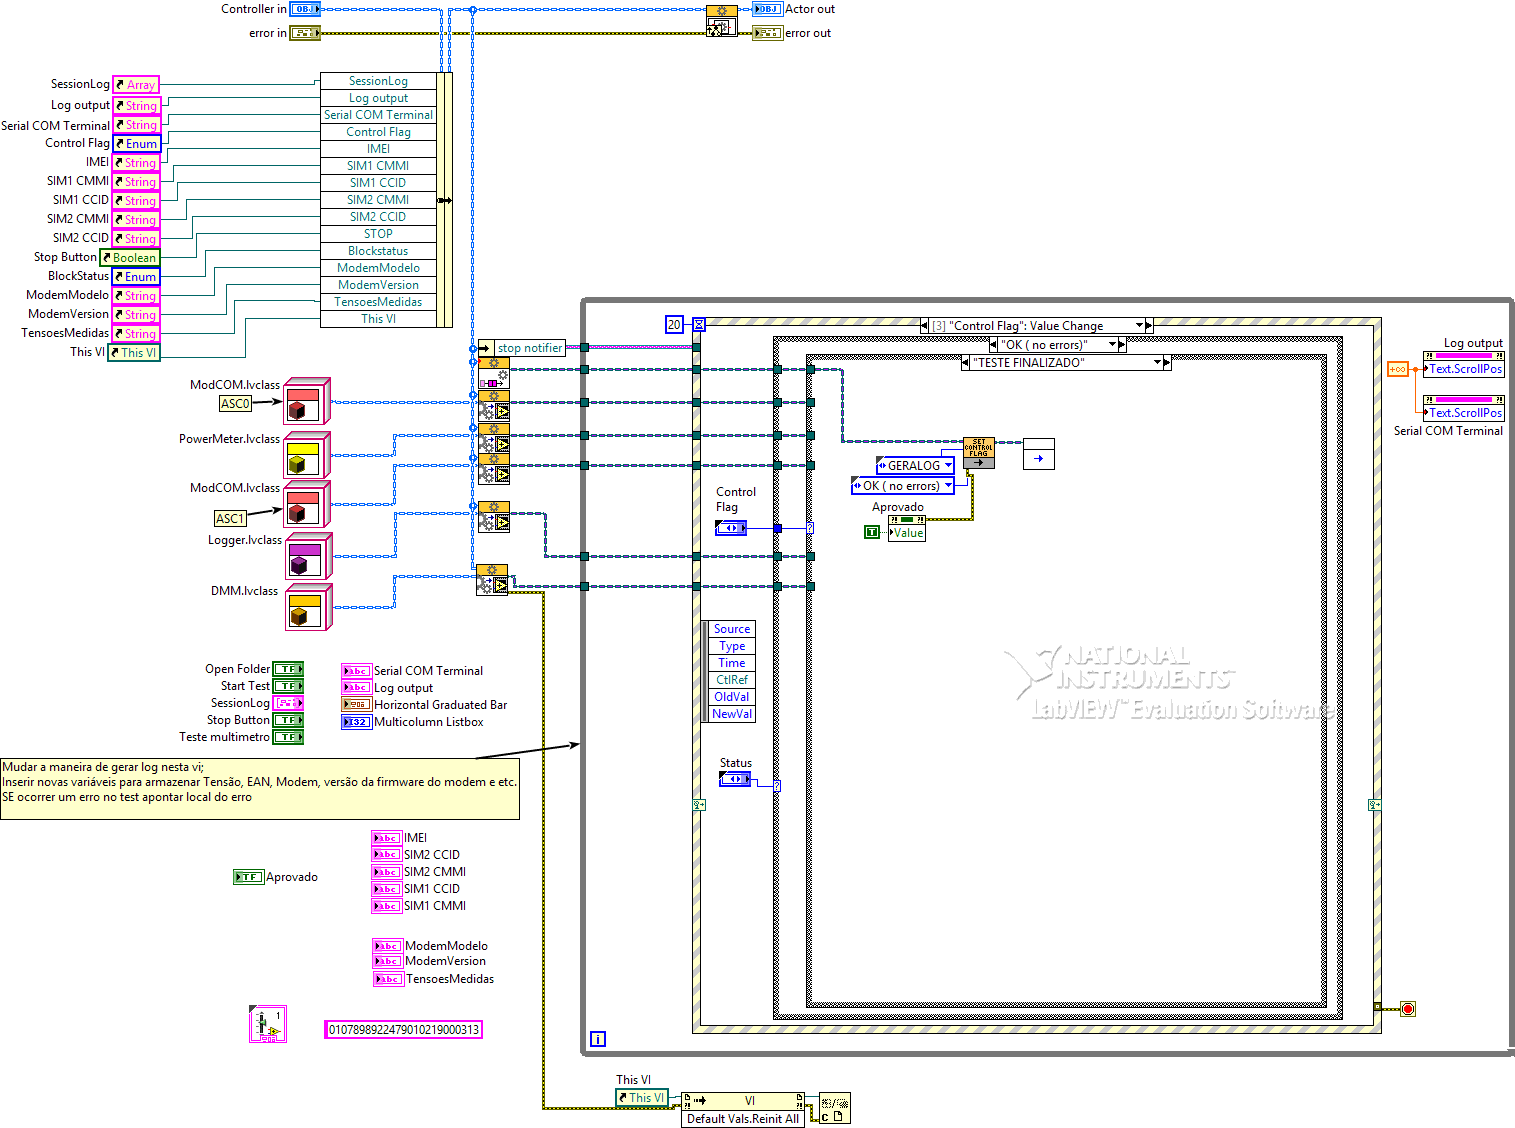
\includegraphics[width=1\linewidth]{lv/controler/Controller_lvclass_Actor_Cored}
                \caption{Diagrama de blocos do \textit{Actor Core.vi} do Controlador}
                \label{fig:cntrlcore}
        \end{figure}
          
        \begin{figure}
                \centering
                \begin{subfigure}[b]{0.45\textwidth}
                    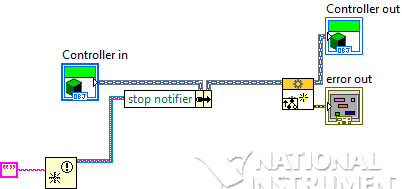
\includegraphics[width=1\linewidth]{lv/controler/Controller_lvclass_Pre_Launch_Initd}
                    \caption{VI de pré-inicialização}
                \end{subfigure}
                \begin{subfigure}[b]{0.45\textwidth}
                    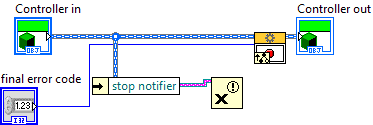
\includegraphics[width=\linewidth]{lv/controler/Controller_lvclass_Stop_Cored}
                    \caption{VI de parada}
                \end{subfigure}
                \caption{Capturas de tela das VI de pré-inicialização e parada do Ator}
                \label{fig:cntrlprestop}
        \end{figure}
        
        \begin{figure}
                \centering
                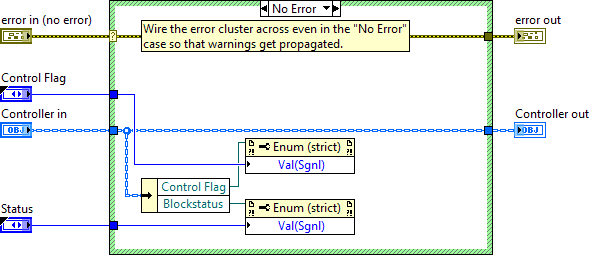
\includegraphics[width=0.9\linewidth]{lv/controler/Controller_lvclass_SET_Control_Flagd}
                \caption{Captura de tela do método interno que recebe a mensagem do bloco de teste executado e seu status de conclusão.}
                \label{fig:cntrlset}
        \end{figure}
        
\section{VI do ator powermeter}
 
    \begin{figure}
        \centering
        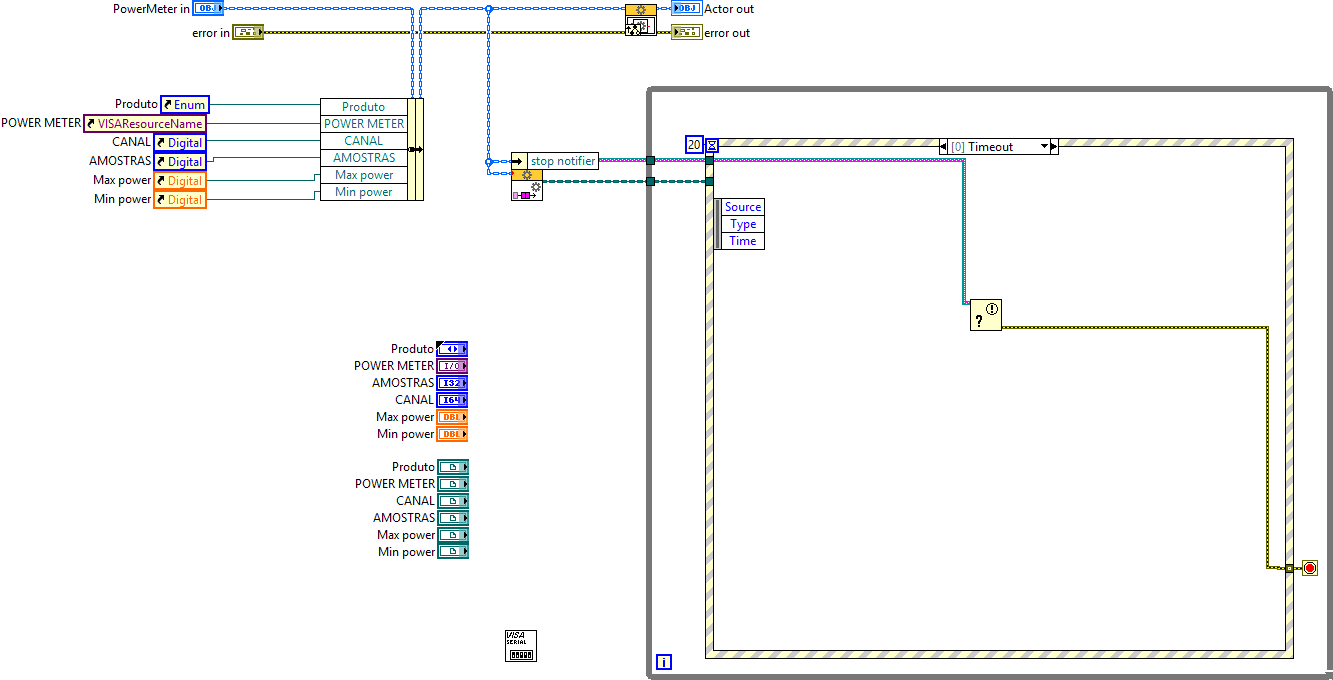
\includegraphics[width=1\linewidth]{lv/pwmtr/PowerMeter_lvclass_Actor_Cored}
        \caption{Captura de tela do Actor Core do Power Meter}
        \label{fig:pwcore}
    \end{figure}
    \begin{figure}
        \centering
        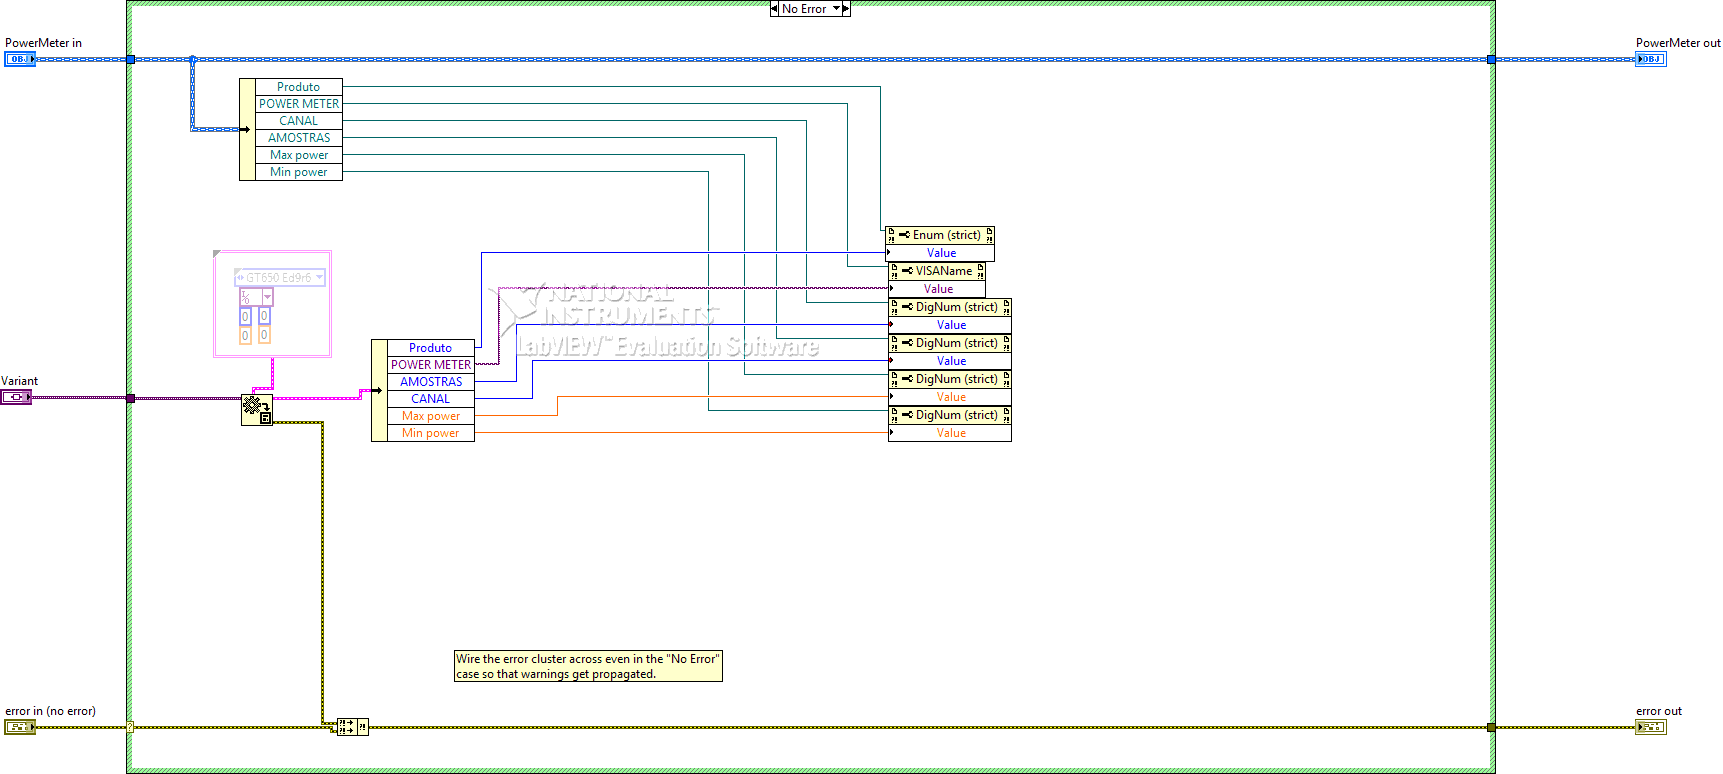
\includegraphics[width=1\linewidth]{lv/pwmtr/PowerMeter_lvclass_SET_PM_Actor_Configd}
        \caption{Captura de tela do Configuração do Power Meter}
        \label{fig:pwconf}
    \end{figure}
    
\section{VI do ator loggger}

    \begin{comment}
                \begin{figure}
                    \centering
                    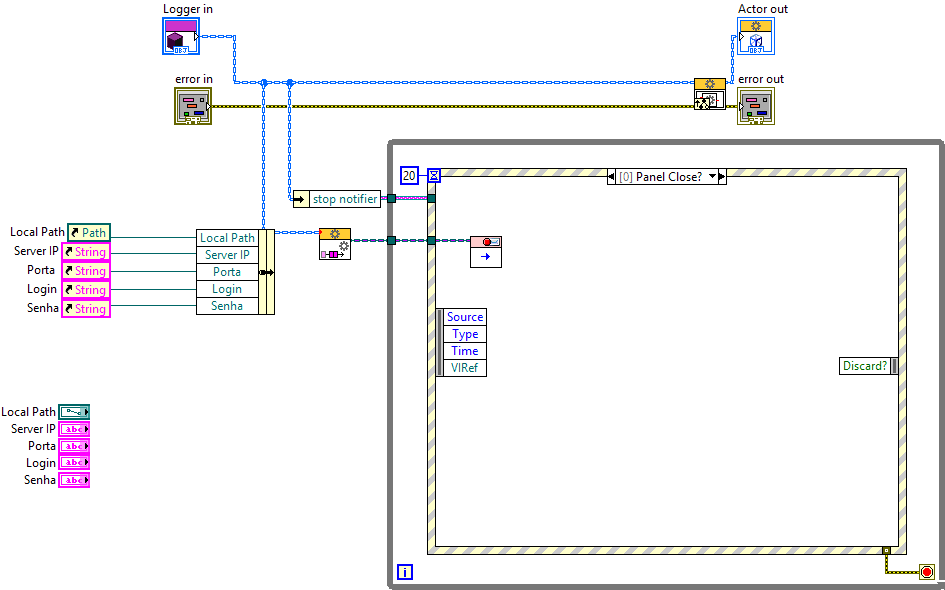
\includegraphics[width=1\linewidth]{lv/log/Logger_lvclass_Actor_Cored}
                    \caption{Captura de tela do Actor Core do Gerador de Log}
                    \label{fig:logcore}
                \end{figure}
                \begin{figure}
                    \centering
                    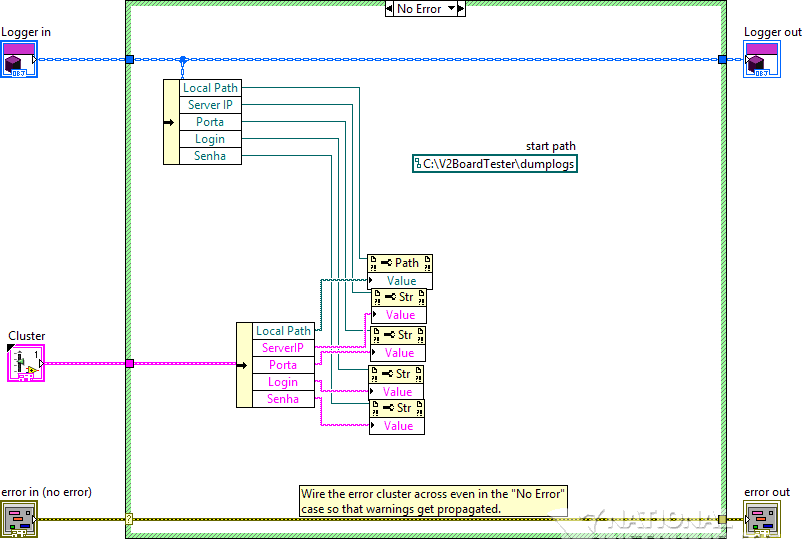
\includegraphics[width=1\linewidth]{lv/log/Logger_lvclass_Configd}
                    \caption{Captura de tela do Configurador Gerador de Log}
                    \label{fig:logconf}
                \end{figure}
        \end{comment}
            
            
            \begin{figure}
                \centering
                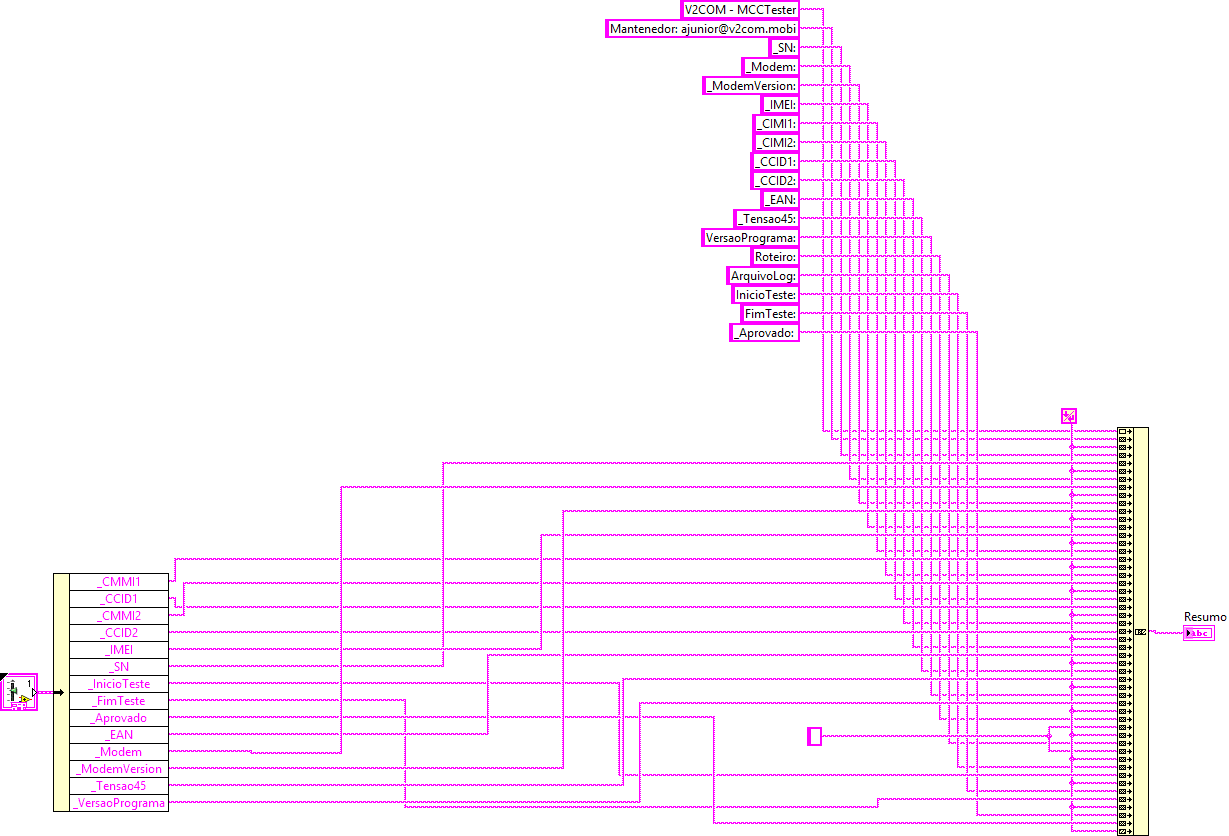
\includegraphics[width=1\linewidth]{lv/log/Logger_lvclass_LogGen_(SubVI)d}
                \caption{Captura de tela do Instrumento virtual de geraçao de log}
                \label{fig:loggen}
            \end{figure}
            \begin{figure}
                \centering
                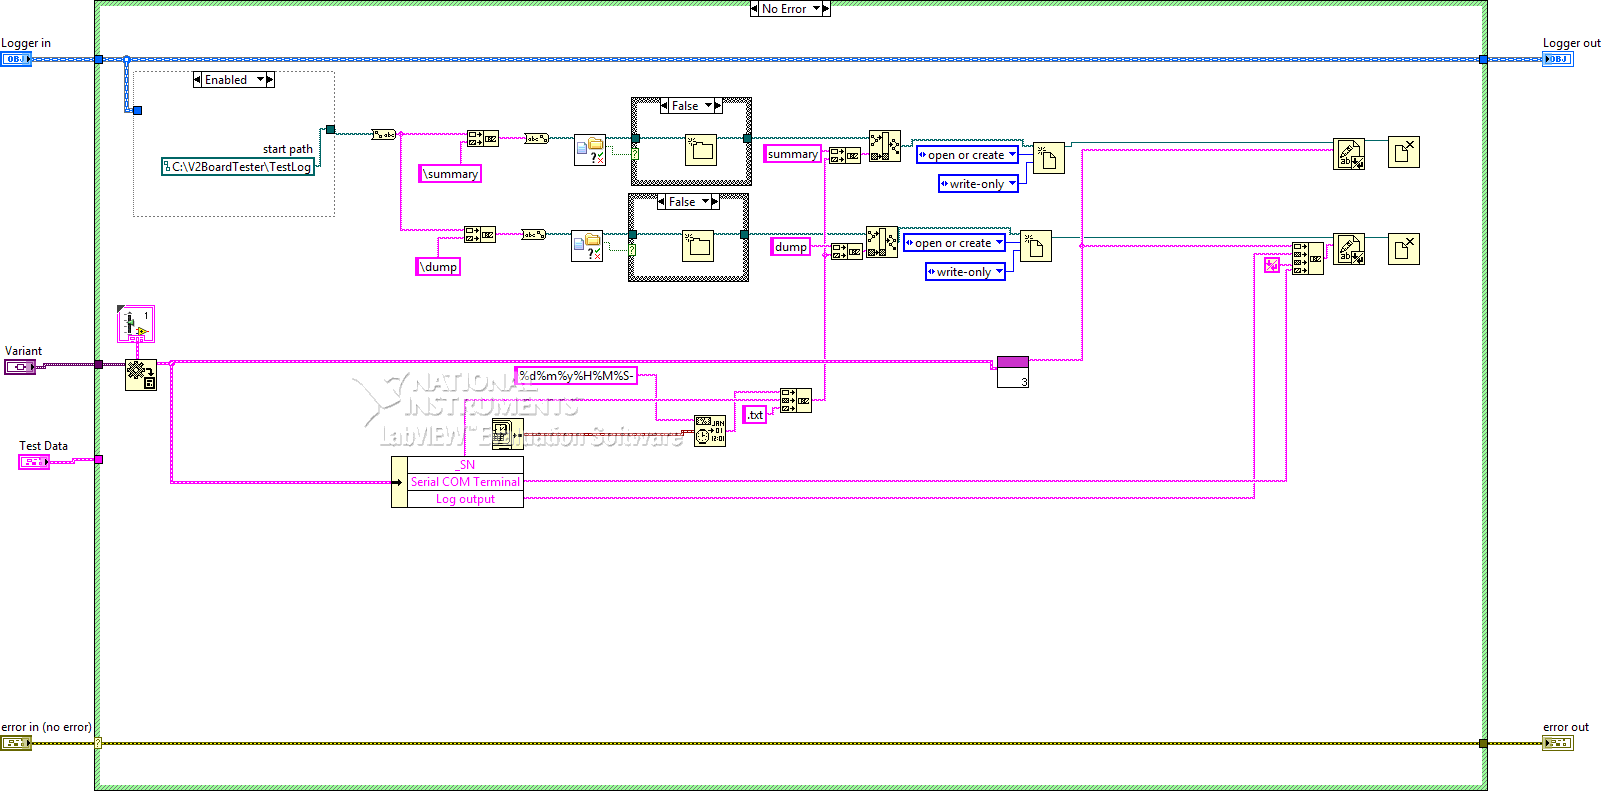
\includegraphics[width=1\linewidth]{lv/log/Logger_lvclass_MakeLogd}
                \caption{Captura de tela do Criador  de Log}
                \label{fig:logmake}
            \end{figure}
            
            
\section{VI do multimetro}
  
            \begin{comment}
            \begin{figure}
                \centering
                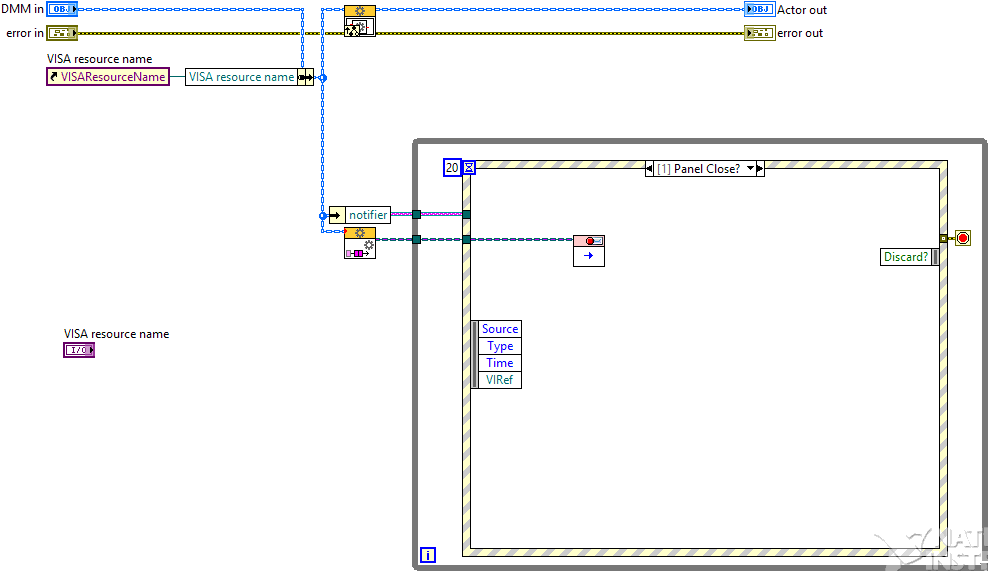
\includegraphics[width=1\linewidth]{lv/dmm/DMM_lvclass_Actor_Cored}
                \caption{Captura de tela do Actor Core do Multimetro}
                \label{fig:dmmcore}
            \end{figure}
            
            \end{comment}
            \begin{figure}
                \centering
                 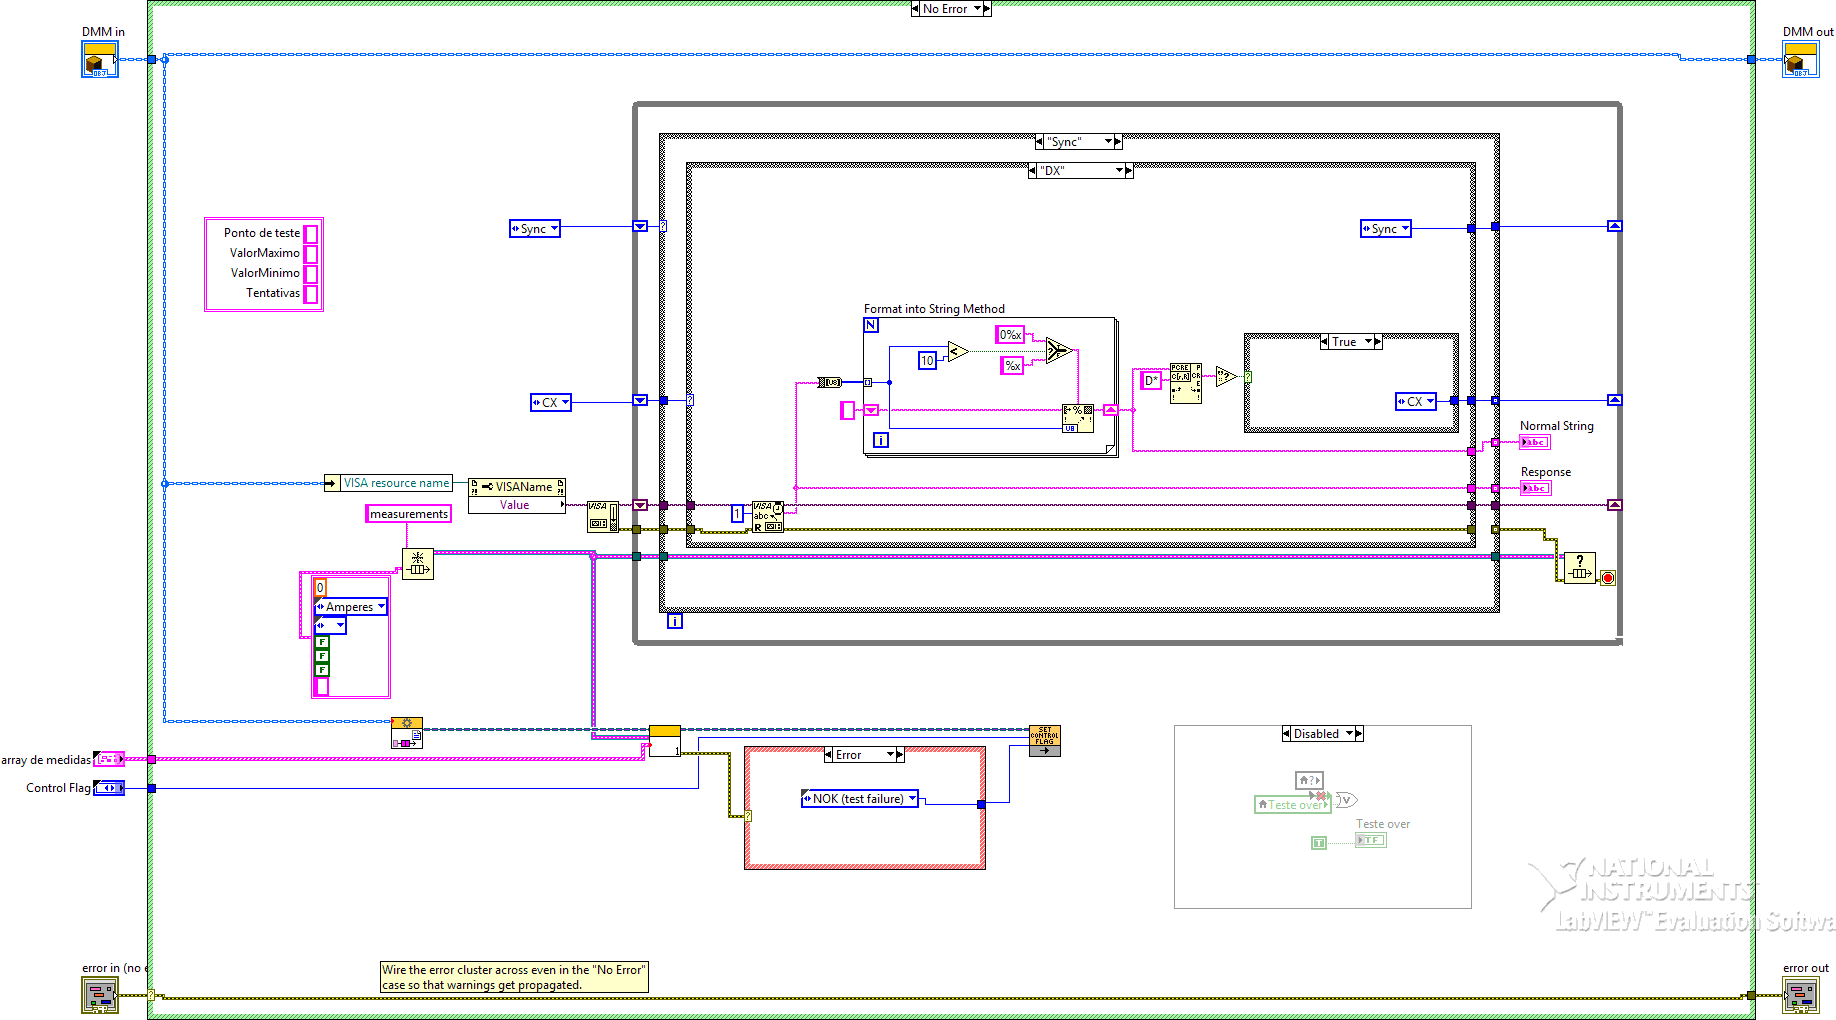
\includegraphics[width=1\linewidth]{lv/dmm/DMM_lvclass_AcquireTestpointsd}
                \caption{Captura de tela do Aquisição de dados pela serial}
                \label{fig:dmmacq}
            \end{figure}
            
            
            \begin{figure}
                \centering
                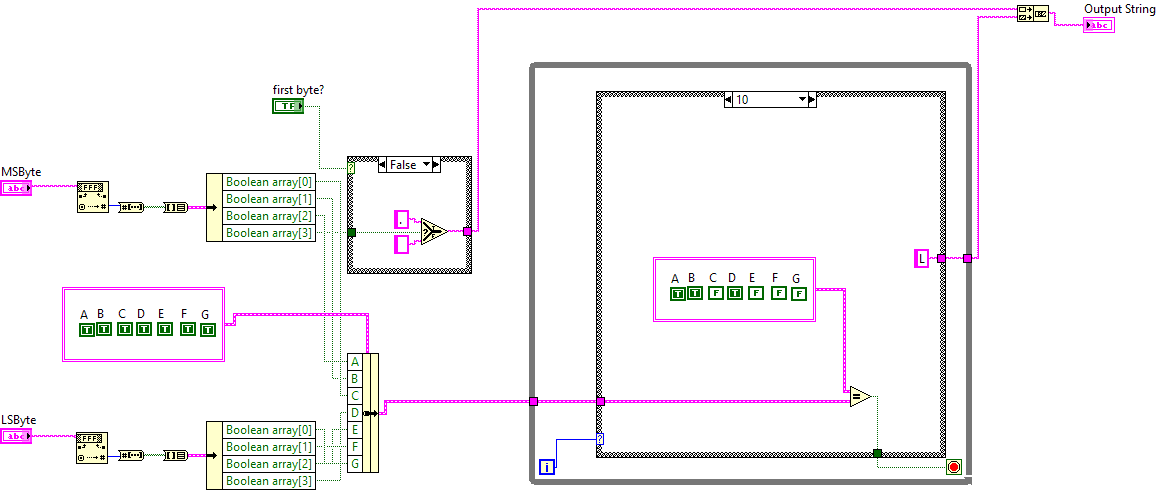
\includegraphics[width=1\linewidth]{lv/dmm/DMM_lvclass_bitcoded}
                \caption{Captura de tela do transformação de 7bitcode em string de números}
                \label{fig:dmmbitcode}
            \end{figure}
            
            
            \begin{figure}
                \centering
                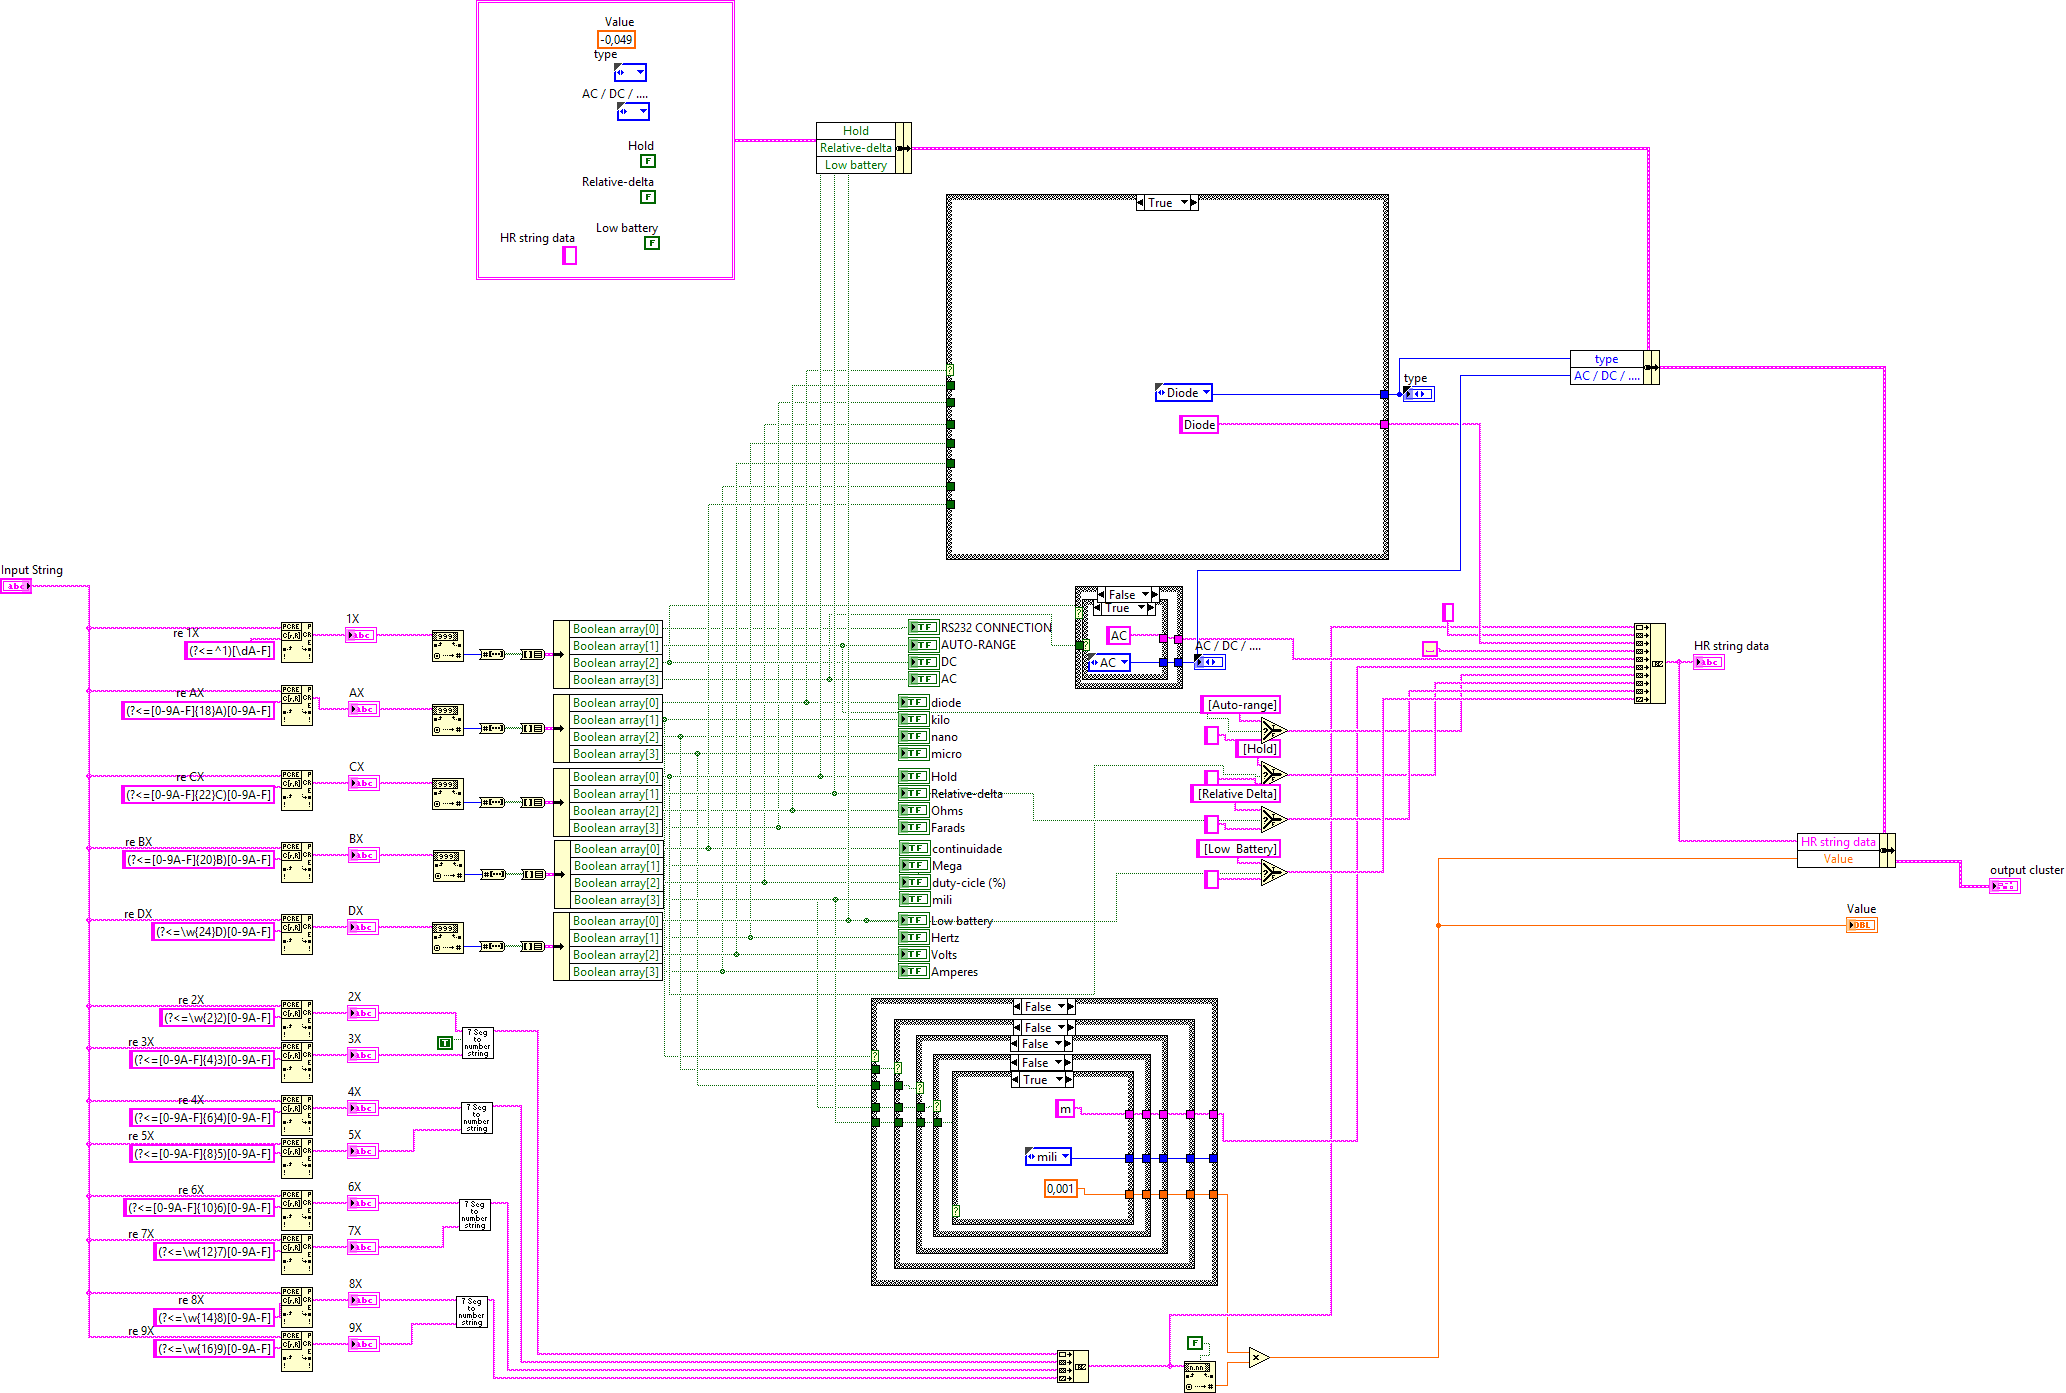
\includegraphics[width=1\linewidth]{lv/dmm/DMM_lvclass_DMM_RS232_14bit_parserd}
                \caption{Captura de tela do Parser da serial}
                \label{fig:dmmparser}
            \end{figure}
            
            
            \begin{figure}
                \centering
                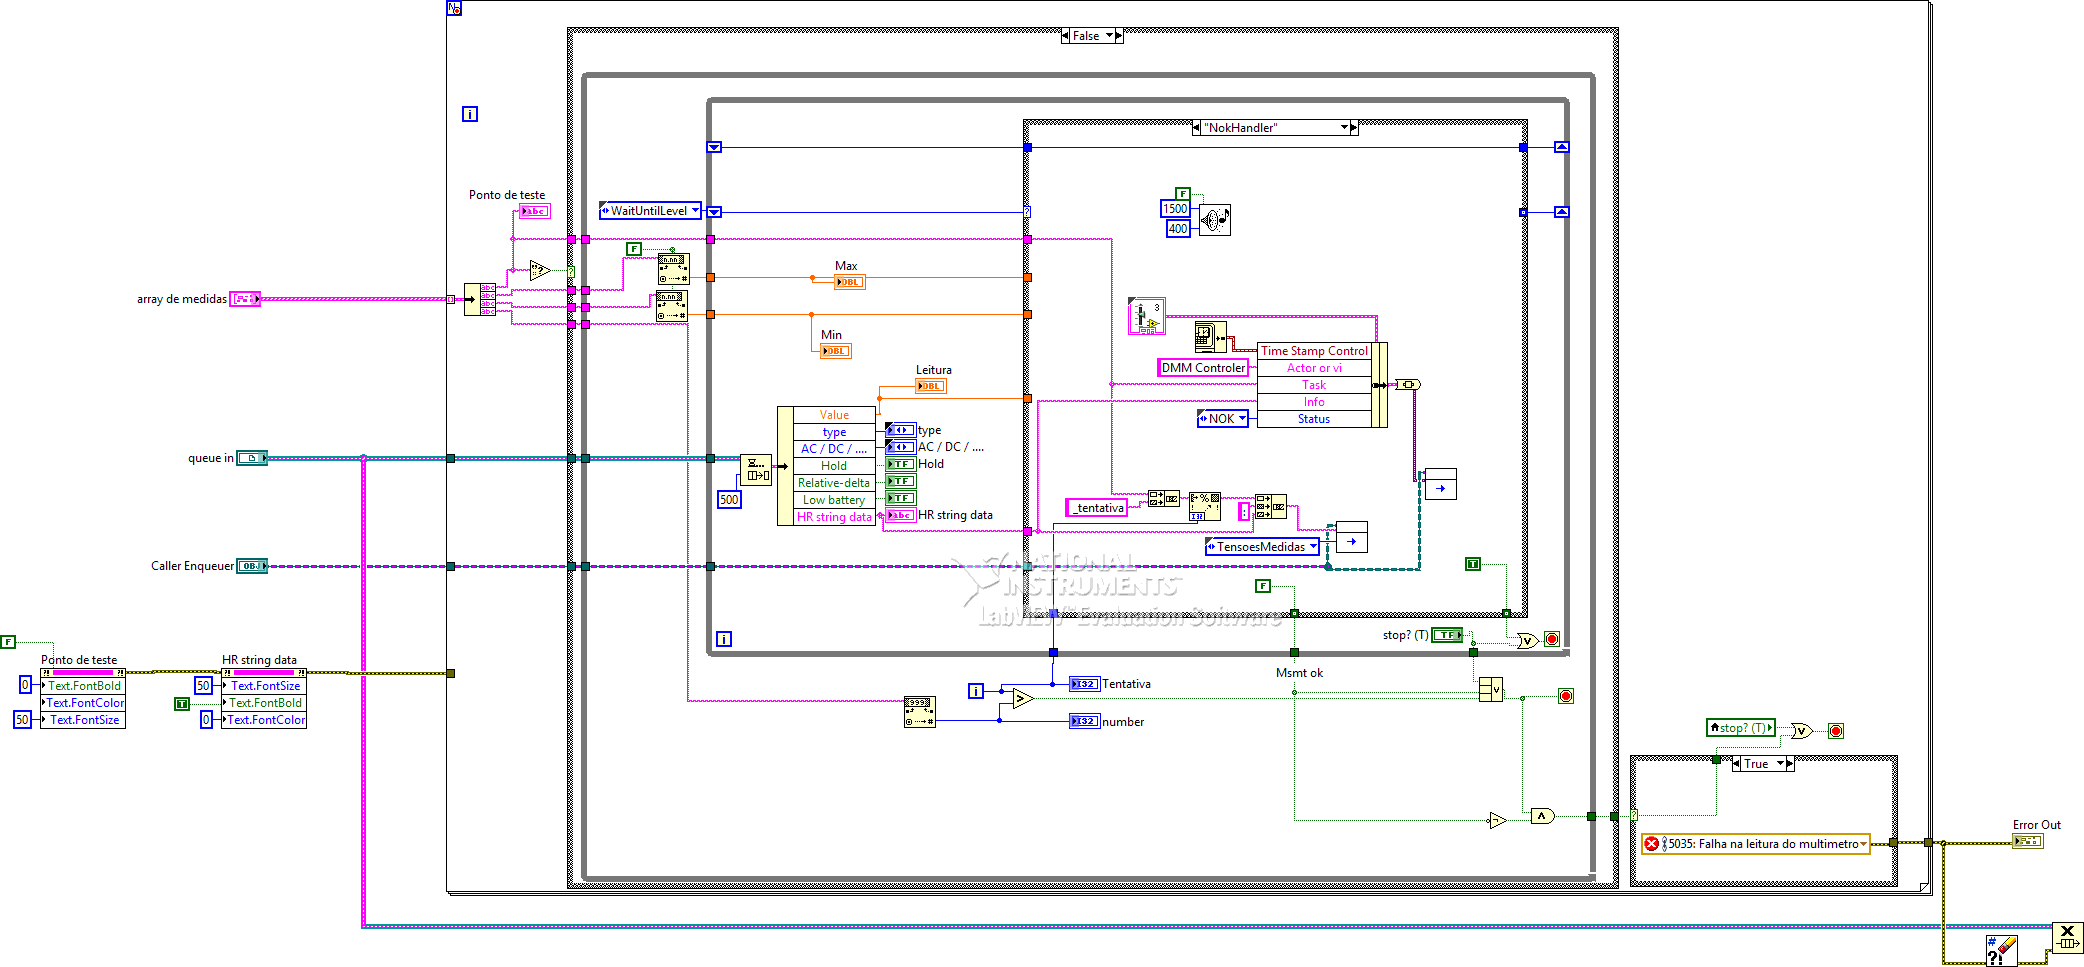
\includegraphics[width=1\linewidth]{lv/dmm/DMM_lvclass_DMM_UI_d}
                \caption{Captura de tela do Diagrama de blocos da interface de usuário}
                \label{fig:dmmfpbd}
            \end{figure}